
%%%%%%%%%%%%%%%
%
% $Autor: Wings $
% $Datum: 2020-02-24 14:30:26Z $
% $Pfad: PythonPackages/Contents/General/Tkinter.tex $
% $Version: 1792 $
%
% !TeX encoding = utf8
% !TeX root = PythonPackages
% !TeX TXS-program:bibliography = txs:///bibtex
%
%
%%%%%%%%%%%%%%%



% Quelle: https://www.heise.de/ratgeber/Python-Einfache-grafische-Bedienoberflaeche-mit-Tkinter-erstellen-4859082.html

\chapter{Package \PYTHON{TKinter}}

\textcolor{red}{
	\begin{itemize}
		\item two description $\rightarrow$ one description
		\item citations!
		\item correct manual
		\item use of \texttt{\textbackslash lstinput}
	\end{itemize}
}

\section{Programmieren mit Python: Einfache grafische Oberfläche mit Tkinter erstellen}

Fenster, Buttons und Menüs machen ein Python-Tool für Nutzer viel attraktiver. Mit der Bibliothek \texttt{Tkinter} geben Sie etwa einem Login-Programm ein Gesicht.

Für den Ersteller eines Python-Skripts ist es oft intuitiv, mit der Kommandozeile zu arbeiten. Aber sobald man das Skript weitergibt und andere Leute damit arbeiten, kommt schnell der Wunsch nach einer grafischen Bedienoberfläche auf. Normale Nutzer sind es gewohnt, Texte in Felder einzugeben, auf Buttons zu klicken und ein Menü am oberen Rand des Programms zu öffnen. Weißer Text auf einem schwarzen Hintergrund wirkt da wie ein Fremdkörper.

In diesem Beispiel versehen Sie ein simples Login-Tool mit einer Bedienoberfläche. Der Nutzer soll seinen Benutzernamen und sein Passwort eingeben und auf einen Login-Button klicken können. Das Programm sagt ihm dann, ob die Daten korrekt waren oder nicht. Eine Menüleiste rundet das Programm ab. So lernen Sie alle wichtigen Grundlagen und Konzepte von Tkinter kennen.

Tkinter ist in Python bereits integriert und bildet die Schnittstelle der Programmiersprache zu Tk, einem kostenlosen Toolkit, um grafische Bedienoberflächen zu gestalten. Tk wurde Ende der 1980er Jahre für die Skriptsprache Tcl entwickelt.

Tkinter in Ihr Python-Programm zu holen ist daher recht einfach:

\medskip

\texttt{\textbackslash PYTHON\{import tkinter as tk\}}

\medskip

Sie müssen vorab keine Pakete mit dem Verwaltungsprogramm pip installieren. Achten sie darauf, \texttt{tkinter} klein zu schreiben, wenn Sie mit der neusten Python-Version arbeiten: Bei Python 2 hieß das Paket noch \texttt{Tkinter}, ab Python 3 heißt es \texttt{tkinter}. Wir importieren die Bibliothek in diesem Beispiel mit dem Zusatz \texttt{as tk}, um mögliche Verwirrungen zu vermeiden und Tkinter einen eigenen Namensraum zu geben. Die Tkinter-Funktionen werden daher mit einem \texttt{tk.} eingeleitet.

%%%%%%%%%%%%%%%%%%%%%%%%%%%%

\subsection{Tk gegen Qt}

Neben Tk könnte man bei Python unter anderem auf das beliebte Framework Qt für eine Bedienoberfläche setzen. Für die Python-Integration sind etwa externe Bibliotheken wie PyQt oder PySide verantwortlich. Qt ist beliebt und es gibt es Dutzende Tutorials im Netz, mit denen komplexe Fensterlayouts möglich sind.

Wir haben uns für dieses Projekt trotzdem für Tk und damit für Tkinter entschieden, weil ein Login-Fenster ein überschaubares Programm ist. Tkinter steht ohne große Vorbereitungen für jedes Python-Projekt bereit. Wer ein Kommandozeilentool schnell mit einer Oberfläche versehen will, für den reicht Tkinter aus – etwa weil die Anwender meckern und Fenster mit Buttons fordern.

%%%%%%%%%%%%%%%%%%%%%%%%%%%%

\subsection{Erstes Fenster erstellen}

Ein erstes Fenster können Sie mit Tkinter in zwei zusätzlichen Zeilen erstellen:

\medskip

\texttt{\textbackslash PYTHON\{programm = tk.Tk()\}}

\texttt{\textbackslash PYTHON\{programm.mainloop()\}}

\medskip

\texttt{\textbackslash PYTHON\{tk.Tk()\}} erstellt quasi das Hauptfenster des Programms und initialisiert das gesamte Tk-Framework. Mit \texttt{\textbackslash PYTHON\{mainloop()\}} schaffen Sie eine Schleife, in der alle Ereignisse verarbeitet werden, die im Fenster passieren. Das Programm hält diese Schleife solange aufrecht, bis der Anwender das Hauptfenster schließt. Die Funktion \texttt{\textbackslash PYTHON\{mainloop()\}} sollte immer am Ende stehen, da sie das aufruft, was Sie vorher gecodet haben.

\begin{figure}
	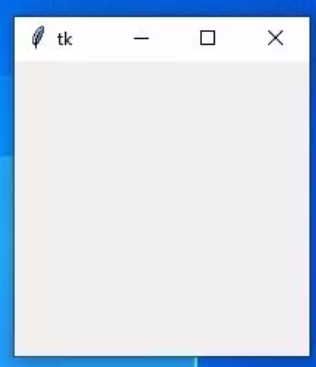
\includegraphics[width=0.5\textwidth]{Tkinter/TkinterFirstWindow}
	\caption{Das erste Fenster ist grau und unspektakulär. Aber ein Fenster.} \label{TkinterFirstWindow}
\end{figure}

Das erste Fenster, siehe \ref{TkinterFirstWindow}, ist mit diesen zwei Zeilen natürlich noch etwas unspektakulär. Graue Fläche, eine Feder als Icon, die an das Tk-Symbol erinnert, tk als Fenstertitel und Schaltflächen fürs Minimieren, Maximieren und Schließen. Aber es ist schon jetzt für viele Anwender der vertraute Look eines Programmfensters.

Nun können Sie ein einfaches Hello-World-Widget hinzufügen. Widgets sind bei Tkinter die Steuerungselemente wie Labels, Buttons, Skalen, Checkboxen, Optionen \HREF{https://docs.python.org/3/library/tkinter.ttk.html\#ttk-widgets}{und viele mehr}. Sie wollen, dass im Fenster der Text Hello World! steht. Das funktioniert mit dem Label-Widget, es zeigt Texte und Bilder an. Erst definieren Sie das Label mit \texttt{\textbackslash PYTHON\{Label()\}}:

\medskip

\texttt{\textbackslash PYTHON\{label = tk.Label(programm, text="Hello World!")\}}

\medskip

Der erste Parameter ist das Elternwidget, in diesem Fall das Hauptfenster. Hinter dem Parameter \texttt{text} steht der Text in Anführungszeichen, den das Label anzeigen soll

\subsection{Hauptfenster erstellen}

Nach diesen Grundlagen gehts nun weiter mit dem echten Programm, einem simplen Login-Fenster für das Einloggen bei heise online. Damit Sie den Überblick behalten, hat es sich bei Tkinter eingebürgert, einzelne Elemente in Klassen zu packen, so auch das Hauptfenster, siehe \ref{TkinterMain}.

\begin{code}
    \lstinputlisting[language=Python,firstline=86, lastline=87]{../code/General/Tkinter/TkinterClass.py} 
    \lstinputlisting[language=Python,firstline=67, lastline=70]{../code/General/Tkinter/TkinterClass.py} 
    \caption{Erstellung eines Hauptfensters}\label{TkinterMain}
\end{code}   




\PYTHON{self} bezieht sich immer auf die Instanz einer Klasse, nicht auf die generelle Klasse. Andere Programmiersprachen geben sowas als versteckten Parameter mit, Python nicht. Sie müssen es nicht unbedingt \PYTHON{self} nennen, das Keyword ist aber eine sehr gebräuchliche Konvention. Um Ihren Code für andere lesbar zu gestalten, sollten Sie sich daran halten. parent bezeichnet das übergeordnete Element. Da es in diesem Fall das Hauptfenster ist, initialisieren Sie es mit None, es gibt schlicht kein übergeordnetes Element.

\PYTHON{\_\_init\_\_} ist in Python eine reservierte Methode. Sie wird dafür genutzt, ein Objekt zu initialisieren, daher der Name. \PYTHON{\_\_init\_\_} ist ähnlich wie ein Konstruktor in C++ oder Java.

In der Methode \PYTHON{\_\_init\_\_} können Sie einige Eigenschaften des Hauptfensters festlegen. Den Titel des Fensters ändern Sie etwa mit einem \PYTHON{self.title(``Heise-Online-Login'')}. Für die Mindestgröße eines Fensters in Pixeln ist \PYTHON{minsize()} verantwortlich:

\medskip

\PYTHON{self.minsize(300, 130)}

\medskip


Der erste Wert legt die Länge fest, der zweite Wert die Höhe. Möchten Sie nicht, dass der Nutzer die Größe des Fensters verändert, schreiben Sie \PYTHON{self.resizable(width=False, height=False)} in die Methode. \PYTHON{width} ist die Länge, \PYTHON{height} die Höhe, \PYTHON{False} beantwortet die Frage, ob der Nutzer Höhe und Länge ändern kann mit Falsch. Weitere Tk-Methoden, die das Hauptfenster beeinflussen, finden Sie online.

\subsection{Gitter erstellen}

Nun konfigurieren Sie das Gitter des Hauptfensters. In diesem Gitter platzieren Sie alle Unterelemente. Das Hauptfenster soll in diesem Beispiel nur als Container dienen, um etwa Frames anzuzeigen, die komplexere Layouts enthalten. Daher konfigurieren Sie nur ein Gitter mit einer Reihe und einer Spalte:

\medskip

\PYTHON{self.grid\_columnconfigure(0, weight=1)}

\PYTHON{self.grid\_rowconfigure(0, weight=1)}

\medskip

\PYTHON{grid\_columnconfigure()} ist für die Spalte verantwortlich, \PYTHON{grid\_rowconfigure()} für die Reihe. Der erste Parameter ist der Index, beginnend bei 0, Sie adressieren also die erste Spalte und die erste Reihe. \PYTHON{weight} legt ein relatives Gewicht der einzelnen Reihen und Spalten zum Rest fest.

Ein Beispiel: Ein Programm hat zwei Spalten. Sie konfigurieren die Spalten so:

\medskip

\PYTHON{self.grid\_columnconfigure(0, weight=1)}

\PYTHON{self.grid\_columnconfigure(1, weight=2)}

\medskip

Die Spalte mit dem Gewicht 2 nimmt sich doppelt so viel Platz wie die Spalte mit dem Gewicht 1. Das wird deutlich, wenn Sie einen leeren Container mit blauem Hintergrund in Spalte 0 platzieren und einen leeren Container mit rotem Hintergrund in Spalte 1. Egal wie groß sie das Fenster ziehen, der rote Container wird dank seines Gewichts immer doppelt so groß sein wie der blaue Container, siehe \ref{TkinterWeights}.


\begin{figure}
    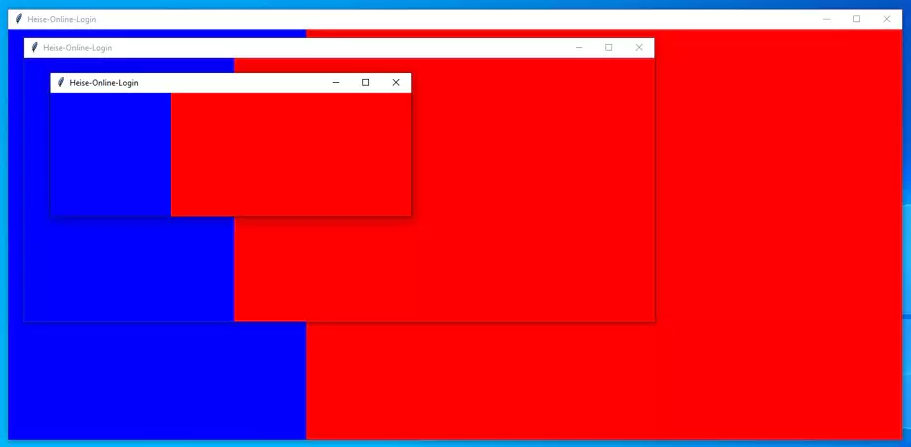
\includegraphics[width=0.5\textwidth]{Images/TKinter/TkinterWeights}
    \caption{Das Gewicht der Spalten beeinflusst ihre Größe.} \label{TkinterWeights}
\end{figure}

%%%%%%%%%%%%%%%%%%%%%%%%%%%%%%%%%%

\subsection{Frame platzieren}

Zurück zum Login-Programm, wo Sie nur eine Spalte und eine Reihe mit demselben Gewicht konfiguriert haben. Der Login soll in einem anderen Frame stattfinden. Ein Frame ist ein Container für Widgets wie Labels, Buttons und so weiter. Für diesen Frame erstellen Sie eine neue Klasse, ähnlich wie beim Hauptfenster:

\medskip

\PYTHON{class Loginframe(tk.Frame):}

\PYTHON{\qquad def \_\_init\_\_(self, parent):}

\PYTHON{}

\PYTHON{tk.Frame.\_\_init\_\_(self, parent)}

\PYTHON{self.parent = parent}

\medskip


Sie haben nun kein \PYTHON{tk.Tk} mehr, sondern \PYTHON{tk.Frame}, da Sie einen Frame benötigen. Im Hauptprogramm definieren Sie nun diesen Frame:

\medskip

\PYTHON{self.loginframe = Loginframe(self)}

\medskip


\begin{figure}
    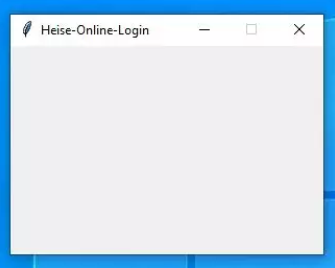
\includegraphics[width=0.5\textwidth]{Images/TKinter/TkinterFrame}
    \caption{Der Titel des Fensters ist schon anders, ansonsten ist das Fenster wüst und leer.} \label{TkinterFrame}
\end{figure}


Dadurch wird deutlich, dass die Instanz des Hauptprogramms (\PYTHON{self}), zum übergeordneten Element für den Loginframe wird (\PYTHON{parent}). Nun müssen Sie diesen Frame noch im Gitter platzieren, sonst wird er nicht angezeigt. Das geht mit \PYTHON{grid()}, indem Sie dem Frame Reihe 0 und Spalte 0 zuweisen:


\medskip

\PYTHON{self.loginframe.grid(row=0, column=0)}

\medskip

Damit sieht das Programm bisher so aus:

\begin{code}
    \lstinputlisting[language=Python,firstline=4, lastline=4]{../code/General/Tkinter/TkinterClass.py} 
    \lstinputlisting[language=Python,firstline=24, lastline=27]{../code/General/Tkinter/TkinterClass.py} 
    \lstinputlisting[language=Python,firstline=67, lastline=79]{../code/General/Tkinter/TkinterClass.py} 
    \lstinputlisting[language=Python,firstline=82, lastline=82]{../code/General/Tkinter/TkinterClass.py} 
    \lstinputlisting[language=Python,firstline=86, lastline=87]{../code/General/Tkinter/TkinterClass.py} 
    \caption{Tkinter Class mit Frame}\label{TkinterFrame}
\end{code}   


\subsection{Widgets erstellen}

Jetzt wird es Zeit, sich Gedanken über die Widgets zu machen, die im Login-Frame erscheinen sollen. Also: Was macht ein Login-Fenster aus? Am wichtigsten sind natürlich die Eingabefelder für den Benutzernamen und das Passwort. Damit der Nutzer auch weiß, welches Eingabefenster für den Benutzernamen und welches für das Passwort gedacht ist, benötigen Sie zwei Labels dafür. Diese Labels können links neben den Eingabefeldern stehen. Ein Beschreibungstext über Labels und Eingabefeldern wäre noch nett, damit der Nutzer weiß, was er da überhaupt tut. Ein Button für den Login darf abschließend unter allen Elementen natürlich nicht fehlen.

Das Schema sieht aus so aus:

\begin{lstlisting}
              Beschreibung-Text
Benutzername-Label    Benutzername-Eingabefeld
    Passwort-Label    Passwort-Eingabefeld
               Login-Button
\end{lstlisting}

\medskip

Damit wissen Sie nun, welche Widgets Sie benötigen und wie sie später platziert werden sollen. Machen Sie sich am Anfang ruhig intensiv Gedanken über das Layout. Später etwas zu ändern ist immer nervig, da Sie dann oft die Position von mehreren Widgets anpassen müssen.

Um die Übersicht zu behalten, verweisen Sie in der Methode \PYTHON{\_\_init\_\_(self , parent)} der Klasse \PYTHON{Loginframe} auf die Methode \PYTHON{Widgets}:

\medskip

\PYTHON{self.Widgets()}

\medskip

Die Methode erstellen Sie anschließend und packen später die Widgets dort rein:
\medskip

\PYTHON{def Widgets(self):}

%%%%%%%%%%%%%%%%%%%%%%%%

\subsection{Beschreibungstext}


Beginnen Sie mit dem Beschreibungstext. Für einen Text mit möglichen Umbrüchen hat Tkinter das Widget \PYTHON{Message()} vorgesehen. Sie können es ähnlich definieren wie das Label im Hello-World-Beispiel:

\medskip

\PYTHON{self.message\_beschreibung = tk.Message(self, text="Gib deine Logindaten für Heise Online ein und drücke dann den Button.", width=240, justify="center")}

\medskip

Der erste Parameter ist wieder das Elternelement, in diesem Fall \PYTHON{self}, also die Instanz des Frames. Hinter \PYTHON{text} verbirgt sich der hardgecodete Text, den Sie später im Fenster sehen möchten. Sie können den Text aber auch in eine Variable auslagern, wenn Sie möchten. \PYTHON{width} gibt die Länge des Widgets an, das müssen Sie nicht unbedingt definieren, ist aber gerade bei statischen Texten sinnvoll, um das Layout zu gestalten. Mit \PYTHON{justify="center"} zentrieren Sie den Text, ansonsten wird er standardmäßig linksbündig angezeigt.

Nun platzieren Sie das Widget in Ihrem Gitter:

\medskip

\PYTHON{self.message\_beschreibung.grid(row=0, column=0, columnspan=2)}

\medskip


Das Widget soll ganz oben stehen, daher startet es in Reihe 0 und Spalte 0. \PYTHON{columnspan=2} gibt an, dass sich dieses Widget über zwei Spalten streckt. Ein Blick auf das vorher visualisierte Layout in Tabellenform ist hier hilfreich.

\subsection{Labels}

Zwei Labels sollen dem Nutzer klarmachen, was er später eintippen soll. Sie können die beiden schnell definieren:

\medskip

\PYTHON{self.label\_benutzername = tk.Label(self, text="Benutzername:")}

\PYTHON{self.label\_passwort = tk.Label(self, text="Passwort:")}

\medskip

Genauso schnell platzieren Sie die Widgets im Gitter:

\medskip

\PYTHON{self.label\_benutzername.grid(row=1, column=0, sticky="e")}

\PYTHON{self.label\_passwort.grid(row=2, column=0, sticky="e")}

\medskip

Das Label für den Benutzernamen steht unter dem vorher angelegten Beschreibungstext, also in Reihe 1. Da es links stehen soll, erhält es die Spalte 0. Das Label für das Passwort steht eine Reihe darunter.

Mit \PYTHON{sticky} lassen Sie Widgets an Rändern kleben. Das \PYTHON{e} steht für east, also für Osten. Ziel ist es, dass die Labels am rechten Rand kleben, während die Eingabefelder eine Spalte weiter am linken Rand kleben. So stehen Sie direkt beieinander. Alle Himmelsrichtungen sind möglich: \PYTHON{n} für Norden, \PYTHON{e} für Osten, \PYTHON{s} für Süden und \PYTHON{w} für Westen. Auch Kombinationen davon: \PYTHON{ew} lässt das Widget am linken und rechten Rand kleben, streckt es also. \PYTHON{nsew} würde versuchen, den gesamten Platz auszufüllen. Die Reihenfolge der Himmelsrichtungen ist dabei egal.

\subsection{Eingabefelder}

Eingabefelder kennt Tkinter unter dem Namen \PYTHON{Entry()}. Hier müssen Sie nicht viel festlegen:

\medskip

\PYTHON{self.entry\_benutzername = tk.Entry(self, width=15)}

\PYTHON{self.entry\_passwort = tk.Entry(self, show="*", width=15)}

\medskip

\PYTHON{width} ist wieder die festgelegte Breite. Spielen Sie ruhig ein wenig mit den Werten herum, um ein gefühl fürs Layout zu erhalten. Das Passwort-Feld kommt noch mit einem \PYTHON{show="*"} als Parameter, damit werden alle eingetippten Buchstaben für den Nutzer durch Sternchen ersetzt -- falls der neugierige Kollege über die Schulter schaut.

Platzieren Sie die Eingabefelder ähnlich wie die zugehörigen Labels:

\medskip

\PYTHON{self.entry\_benutzername.grid(row=1, column=1, sticky="w")}

\PYTHON{self.entry\_passwort.grid(row=2, column=1, sticky="w")}       

\medskip

Auch sie erscheinen unter dem Beschreibungstext, aber wegen dem Parameter \PYTHON{column=1} stehen Sie nun rechts neben den zugehörigen Labels. \PYTHON{sticky="w"} packt die Eingabefelder in den Westen, tackert sie also am linken Rand fest.


%%%%%%%%%%%%%%%%%%%%%

\subsection{Button}

Der Button ist das wichtigste Element in diesem Ensemble, schließlich sorgt er für weitere Aktionen, wenn der Nutzer darauf klickt:

\medskip

\PYTHON{self.button\_login = tk.Button(self, text="Einloggen", command = self.Button\_login\_geklickt)}

\medskip

Der Paramater \PYTHON{text} bestimmt, was auf dem Button stehen soll: Einloggen. \PYTHON{command} gibt an, was bei einem Klick passieren soll. Hier verweist der Klick auf die Methode \PYTHON{Button\_login\_geklickt}, die noch nicht existiert.

Bevor Sie der Aktion einen Sinn geben, packen Sie den Button ins Gitter:

\medskip

\PYTHON{self.button\_login.grid(row=3, column=0, columnspan=2)}

\medskip

Er steht unter den Labels und Einagbefeldern (\PYTHON{row=3}), beginnt in der ersten Spalte (column=0) und belegt zwei Spalten (\PYTHON{columnspan=2}).

Und damit haben Sie eine Fläche erstellt, das wie ein echtes Login-Fenster aussieht. Der Code für die Widgets ist überschaubar, siehe \ref{TkinterWidget}.


\begin{code}
    \lstinputlisting[language=Python,firstline=30, lastline=47]{../code/General/Tkinter/TkinterClass.py} 
    \caption{Widget für die Tkinter Class}\label{TkinterWidget}
\end{code}   

%%%%%%%%%%%%%%%%%%%%%%%%%%%%%%%%

\subsection{Kosmetik}

\begin{figure}
    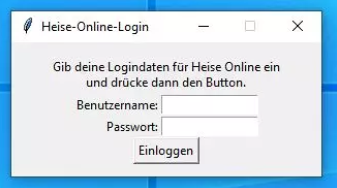
\includegraphics[width=0.5\textwidth]{Images/TKinter/TkinterLogin}
    \caption{Sieht aus wie ein Login-Fenster, tut aber noch nichts.} \label{TkinterLogin}
\end{figure}


Die grundlegenden Widgets sind da, aber etwas Kosmetik fehlt noch. So muss der Nutzer immer erst in die Eingabefelder klicken, damit er loslegen kann. Ein \PYTHON{self.entry\_benutzername.focus()} setzt den Fokus sofort auf das Feld für den Benutzernamen. \PYTHON{1337H4xxx00R97} kann also sofort anfangen, seinen Namen einzutippen.

Dann wäre es noch nett, wenn der Nutzer nicht nur auf den Button klicken kann, sondern einfach die Entertaste drückt, wenn er fertig ist. Das geht mit \PYTHON{bind()}:

\medskip

\PYTHON{self.master.bind("<Return>", self.Button\_login\_geklickt)}

\medskip

Es bindet die Tastenkombination im ersten Parameter (\PYTHON{<Return>}, also Enter) an einen Befehl. In diesem Fall ist es derselbe Befehl, der auch beim Klick auf den Button ausgeführt wird.

Aber: Sie können so viel eingeben und rumdrücken wie Sie möchten, noch tut sich da nix. Als nächstes fügen Sie dem Programm echte Funktionen hinzu.

\subsection{Button klickbar machen}

Der Button verweist beim Klick auf die Methode \PYTHON{Button\_login\_geklickt}: \PYTHON{def Button\_login\_geklickt(self, event=None):}. Dort findet der Login mit den Daten aus den Eingabefeldern statt. Den Parameter \PYTHON{event=None} benötigen Sie, weil Sie vorher mit \PYTHON{bind()} ein Event an diese Methode gebunden haben, nämlich das Drücken der Entertaste. Dieses Event wird immer versteckt weitergereicht. In diesem Beispiel würde nur \PYTHON{event} als Parameter ausreichen, mit \PYTHON{event=None} definieren Sie es aber vorher. Mit \PYTHON{print(event)} in der Methode können Sie sich etwa weitere Infos zu dem Tastendruck anzeigen lassen.

Mit \PYTHON{get()} holen Sie die Eingaben des Nutzers aus den Feldern:

\medskip

\PYTHON{self.benutzername = self.entry\_benutzername.get()}

\PYTHON{self.passwort = self.entry\_passwort.get()}

\medskip

Damit können Sie nun weiterarbeiten und sich bei heise online einloggen. Wir nutzen dafür den Login über die externe Bibliothek Requests. Sie müssen die Bibliothek vorher installieren, etwa mit dem Paketverwalter pip:

\medskip

\SHELL{pip install requests}

\medskip


Der Befehl \PYTHON{import} holt die Bibliothek ins Programm:

\medskip



\PYTHON{import requests}


\subsection{Fake-Browser und Login-Daten}

Anschließend definieren Sie einen Fake-Browser in einem Dictionary, um auf die Daten zugreifen zu können:

\medskip

\PYTHON{self.fake\_browser =\{"{}User-Agent":"Mozilla/5.0 (Windows NT 10.0; Win64; x64; rv:77.0) Gecko/20100101 Firefox/77.0"\}}

\medskip

Der User-Agent enthält Daten über den Browser und dem verwendeten System und wird an Webseiten geschickt, wenn Sie eine aufrufen. Ihren eigenen User-Agent sehen Sie etwa auf \URL{http://wieistmeinuseragent.de}. Ihr Python-Programm tut dann so, als wäre es dieser User-Agent.

Die Daten für den Login speichern Sie in einem weiteren Dictionary:

\medskip

\PYTHON{self.login\_daten = \{"{}username":self.benutzername, "password":self.passwort, "{}action":"/sso/login/login"\}}

\medskip

Um sich an einer Website einzuloggen, müssen Sie sie vorher analysieren. Bei heise online passiert das über die Seite \URL{https://www.heise.de/sso/login/login} und einer POST-Methode mit der Aktion \PYTHON{/sso/login/login}. Wie genau Sie solche Feinheiten entdecken und sich richtig anmelden, haben wir in einem anderen Artikel ausführlich aufgeschrieben.

Zusammengenommen funktioniert der Login dann so:

\medskip

\PYTHON{self.login = requests.Session().post(url="https://www.heise.de/sso/login/login", data=self.login\_daten, headers=self.fake\_browser)}

\medskip

Mit \PYTHON{requests.Session()} erstellen sie eine Session, das bedeutet, dass etwa Cookies gespeichert werden und Sie später mit aktivem Login andere Seiten aufrufen können. \PYTHON{post()} steht für die HTML-Methode POST, die \PYTHON{url} ist die heise-Login-Seite, data enthält die vorher festgelegten Login-Daten und in headers geben Sie den Fake-Browser als User-Agent mit.

%%%%%%%%%%%%%%%%%%%%%%%%%%%%%%%%%%%%%

\subsection{Fehlermeldung}

Das war der Login. Aber er ist noch recht unsichtbar, schließlich tun Sie damit noch nichts. Eine Fehlermeldung ist hilfreich, falls der Nutzer falsche Daten eingibt. Sie erkennen einen fehlgeschlagenen Login daran, dass im Text von \PYTHON{self.login} der Satz ``Der Benutzername oder das Passwort ist falsch.'' auftaucht. Das fragen Sie ab:

\medskip

\PYTHON{if "Der Benutzername oder das Passwort ist falsch." in self.login.text:}

\medskip

Wenn dieser Text vorkommt, soll sich die Beschreibung ändern und den Nutzer auf den Fehler aufmerksam machen. Anschließend kann er es nochmal probieren. Das geht etwa so:

\medskip

\PYTHON{self.message\_ beschreibung.config(text="Fehler: Der Benutzername oder das Passwort ist falsch.", width=160, fg="red")}

\medskip

\begin{figure}
    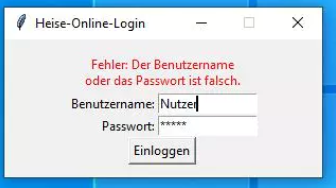
\includegraphics[width=0.5\textwidth]{Images/TKinter/TkinterError}
    \caption{Da ist was schiefgelaufen.} \label{TkinterError}
\end{figure}




Das Programm leitet die Daten nur durch und speichert sie nicht. Die Fehlermeldung wird anhand der Reaktion der Website erstellt, siehe \ref{TkinterError}. Sollte sich also die Fehlernachricht auf heise online ändern, würde das Skript nicht mehr funktionieren.

Mit \PYTHON{config()} ändern Sie die Eigenschaften des Widgets und passen den Text an. Auch die Breite ändern Sie und die Textfarbe setzen Sie mit fg für foreground, also Vordergrund, auf red, als rot. Ist ja ein Fehler. Parameter, die Sie nicht änder,n bleiben erhalten -- wie etwa \PYTHON{justify="center"}.

Nun müssen Sie noch entscheiden, was passiert, wenn der Nutzer sich korrekt einloggt. Sie können etwa ein neues Fenster aufrufen und den Login-Frame zerstören. Sie benötigen ihn ja nicht mehr.

%%%%%%%%%%%%%%%%%%%%%%%%%%%%%%%

\subsection{Korrekter Login}


Für das neue Fenster erstellen Sie eine neue Klasse namens \PYTHON{Loginerfolg} mit einer simplen Nachricht, siehe \ref{TkinterLoginErfolg}:

\begin{code}
    \lstinputlisting[language=Python,firstline=14, lastline=22]{../code/General/Tkinter/TkinterClass.py} 
    \caption{Klasse \PYTHON{Loginerfolg}}\label{TkinterLoginErfolg}
\end{code}   


Alle Elemente daraus dürften Ihnen bekannt vorkommen.

Das neue Fenster definieren Sie zudem im Hauptprogramm, in der Klasse Programm:

\medskip

\PYTHON{self.loginerfolg = Loginerfolg(self)}

\medskip

Die Idee: Sie zerstören das Loginfenster, verweisen dann über das Hauptprogramm auf den Frame Loginerfolg. Gehen Sie dafür zurück in die Klasse Loginframe und in die Methode \PYTHON{Button\_login\_geklickt}. Dort legen Sie eine Alternative zum gescheiterten Login an:

\medskip

\PYTHON{else:}

\PYTHON{\qquad self.destroy()}

\PYTHON{\qquad self.parent.loginerfolg.grid(row=0, column=0)}

\medskip


\begin{figure}
    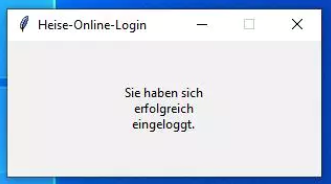
\includegraphics[width=0.5\textwidth]{Images/TKinter/TkinterLoginOk}
    \caption{Erfolg: Der Login hat geklappt.} \label{TkinterLoginOk}
\end{figure}



\PYTHON{self.destroy()} schließt einen Frame, in diesem Fall die aktuelle Instanz des Frames. \PYTHON{self.parent.loginerfolg.grid()} verweist auf das übergeordnete Element, also auf die Klasse \PYTHON{Programm}. Genau für so einen Fall haben Sie in der Methode \PYTHON{\_\_init\_\_} der Klasse \PYTHON{Loginframe} \PYTHON{self.parent = parent} definiert. Die Klasse \PYTHON{Programm} kennt auch schon \PYTHON{loginerfolg}, denn das haben Sie vorher dort definiert: \PYTHON{self.loginerfolg = Loginerfolg(self)}. Mit \PYTHON{grid()} setzen Sie schließlich das neue Fenster \PYTHON{Loginerfolg} im Hauptfenster ein und machen es für den Nutzer sichtbar, siehe \ref{TkinterLoginOk}.

Es kann am Anfang ein wenig verwirrend sein, da Sie hier zwischen den Klassen hin und her springen. Vereinfacht gesagt geht der Übergang so: Das Loginfenster zerstört sich selbst und ruft über das Hauptprogramm die Erfolgsnachricht in einem anderen Fenster auf.

%%%%%%%%%%%%%%%%%%%%%%%%%%%%%%

\subsection{Menüleiste erstellen}


Den Hauptteil haben Sie damit abgeschlossen, der Login funktioniert. Aber ein Programm kann ja immer schöner werden. Sie können etwa eine Menüleiste erstellen, über die der Nutzer das Programm beenden kann.

Erstellen Sie eine neue Klasse:

\medskip

\PYTHON{class Menu\_Leiste(tk.Menu):}

\PYTHON{\qquad def \_\_init\_\_(self, parent):}

\PYTHON{\qquad \qquad tk.Menu.\_\_init\_\_(self, parent)}

\medskip
	           
Sieht bekannt aus, unterscheidet sich von den anderen Klassen eigentlich nur über das \PYTHON{tk.Menu}, es ist ja kein Frame (\PYTHON{tk.Frame}) und auch kein Hauptfenster (\PYTHON{tk.Tk}). Es soll die Menüleiste für alle Fenster werden, daher fügen Sie in der Klasse Programm diesen Eintrag hinzu:

\medskip

\PYTHON{self.config(menu=Menu\_Leiste(self))}

\medskip

Zurück zur Klasse \PYTHON{Menu\_Leiste}. Nun spendieren Sie der Leiste ein Datei-Menü:

\medskip

\PYTHON{Datei\_Menu = tk.Menu(self, tearoff=False)}

\medskip

\PYTHON{tearoff} ist auf \PYTHON{False} gesetzt. Wäre der Parameter \PYTHON{True}, würde das Menü eine gestrichelte Leiste oben erhalten, mit der der Nutzer das Menü loslösen und verschieben kann. Diese Funktion kann nützlich sein, hier verzichten wir darauf.

Das Datei-Menü erhält nun mit der Funktion \PYTHON{add\_cascade()} ein neues Untermenü:

\medskip

\PYTHON{self.add\_cascade(label = "Datei", menu = Datei\_Menu)}

\medskip

label legt den Namen fest, Datei, das Datei-Menü verknüpfen Sie über den Parameter \PYTHON{menu}.

Nun fügen Sie dem Menü den ersten Befehl hinzu mit der Funktion \PYTHON{add\_command()}:

\medskip


\PYTHON{Datei\_Menu.add\_command(label = "Beenden", command = self.quit, accelerator="Alt+F4")}

\medskip

\begin{figure}
    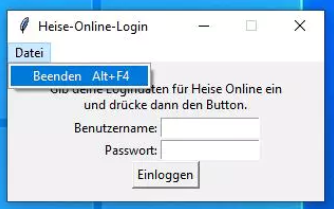
\includegraphics[width=0.5\textwidth]{Images/TKinter/TkinterMenu}
    \caption{Ein gewohntes Menü mit einem gewohnten Befehl.} \label{TkinterMenu}
\end{figure}

\PYTHON{label} ist der Name des Befehls, \PYTHON{accelerator} fügt einen Text rechts neben dem Label hinzu. Sie können es etwa nutzen, um Tastenkombinationen für den Befehl anzuzeigen, siehe \ref{TkinterMenu}. \PYTHON{command} enthält den Befehl, hier \PYTHON{self.quit}, was das gesamte Programm beendet.

Auf diese Weise können Sie noch weitere Einträge und Befehle hinzufügen, um etwa andere Fenster zu öffnen oder Einstellungen zu ändern. Der gesamte Code für das kleine Beispielprogramm ist in \ref{TkinterComplete} dargestellt.

\begin{code}
    \lstinputlisting[language=Python]{../code/General/Tkinter/TkinterClass.py} 
    \caption{Klasse \PYTHON{Loginerfolg}}\label{TkinterComplete}
\end{code}   

\subsection{Fazit}

Viele Möglichkeiten sind bei Tkinter selbsterklären, wenn man es mindestens einmal gemacht hat. Fenster erstellen Sie immer wieder gleich, Widgets lassen sich auf ähnliche Arten bearbeiten und Menüpunkte kann man schnell hinzufügen. Wer nicht weiterkommt, findet über Google viele beantwortete Fragen aus der Community.

Bei komplexeren Layouts und Programmen kann man aber den Überblick verlieren. Daher ist es wichtig, seinen Klassen und Methoden eindeutige Namen zu geben. Für eine schnelle Umsetzung eines einfachen Konsolentools ist Tkinter aber gut geeignet und ist eine Alternativen zu Framworks wie Qt.


\section{Package Tkinter}

\subsection{Introduction}

Tkinter is the standard GUI (Graphical User Interface) library for Python. Python, being easy to use and having a readable syntax, is a popular choice for beginners and experts alike. Tkinter provides a fast and simple way to create GUI applications. It is a thin object-oriented layer on top of Tcl/Tk.

This report aims to provide a comprehensive overview of the Tkinter package, including its description, installation process, and various examples demonstrating its usage in different scenarios. Additionally, further reading resources will be suggested for those interested in diving deeper into the Tkinter library. 

The version of the Tkinter package used here is 8.6 which is supposed to install together during the 1st Python installation. This package is used for creating Graphical User Interface (GUI) for Desktop Applications. With the help of Tkinter developing desktop applications is not a tough task thus it is a good way to start creating simple projects in Python.. Tkinter functions are explained in the upcoming sections.

\subsection{Description}

Tkinter in Python helps in creating GUI Applications with minimum hassle. Among various GUI Frameworks, Tkinter is the only framework that is built-in into Python's Standard Library.

An important feature in favor of Tkinter is that it is cross-platform, so the same code can easily work on Windows, macOS, and Linux. Since Tkinter is a lightweight module, it usually comes as part of the standard Python installation, so you don't have to install it separately.

Tkinter is one of the most common and accessible libraries for building GUIs in Python. Tkinter provides various controls, such as buttons, labels, and text boxes, used in a desktop application. It is event-driven, meaning it waits for the user to take an action, such as pressing a button or entering text, and reacts accordingly.

\subsubsection{What are Tcl, Tk, and Tkinter?}

\begin{itemize}
    
    \item Tkinter is based upon the Tk toolkit, which was originally designed for the Tool Command Language (Tcl). As Tk is very popular thus it has been ported to a variety of other scripting languages, including Perl (Perl/Tk), Ruby (Ruby/Tk), and Python (Tkinter).
    
    \item The wide variety of widgets, portability, and flexibility of Tk makes it the right tool which can be used to design and implement a wide variety of simple and complex projects.
    
    \item Python with Tkinter provides a faster and more efficient way to build useful desktop applications that would have taken much time if you had to program directly in C/C++ with the help of native OS system libraries.
    
\end{itemize}

\subsubsection{Advantages of Tkinter}

\begin{itemize}
    \item \textbf{Layered Design:}
    Tkinter is structured in a layered fashion, drawing on the strengths of the established TK library. This design choice has endowed Tkinter with the seasoned benefits of a mature GUI toolkit, enhancing its stability and dependability right from the start. Unlike a ground-up development, this approach ensured that Tkinter was robust from its early versions. Additionally, the transition from Tcl/Tk to Tkinter is straightforward, allowing programmers familiar with Tk to adapt to Tkinter with minimal effort.
    
    \item \textbf{User-Friendly:}
    The design of Tkinter aligns with the intuitive and straightforward ethos of Python, making it an accessible choice for GUI development. It simplifies complex operations into user-friendly methods, embodying Python's rapid prototyping capabilities.
    
    \item \textbf{Portability:}
    Tkinter exemplifies cross-platform compatibility, as Python scripts utilizing Tkinter can be seamlessly transferred across different environments without needing alterations. It supports all major operating systems where Python is available, such as Microsoft Windows, X Windows, and macOS. This universality is a significant edge over other libraries that might be limited to specific systems. Furthermore, Tkinter ensures that applications adhere to the native look and feel of the operating system they are running on.
    
    \item \textbf{Availability:}
    Tkinter is bundled with all standard Python distributions, eliminating the need for additional modules to develop Tkinter-based applications. This built-in availability makes it an immediately accessible option for Python developers, streamlining the process of creating and deploying GUI applications.
    
    \item \textbf{Rich Set of Widgets:}Includes standard widgets like buttons, labels, text boxes, check buttons, etc.
    
    \item \textbf{Lightweight:} Comes pre-installed with Python, requiring no additional installation to start building GUI applications.
\end{itemize}

\subsubsection{Disadvantages of Tkinter}

Mostly the concern of Tkinter is the layered design of Tkinter that may impact performance, potentially slowing down execution. This could pose issues for older, less powerful computers. However, the majority of contemporary machines are equipped to handle the additional processing demands within acceptable time frames. When performance is a priority, it is crucial to ensure that the code is written with maximum efficiency in mind.

\subsection{Installation}

Tkinter comes pre-installed with Python, so there's usually no need to install anything to start developing GUI applications. However, if it's missing for any reason, it can typically be installed:

\subsubsection{Python Version Support}

Due to pre-installed feature, Tkinter officially supports a range of Python versions, from Python 2 to Python 3.

Tkinter comes pre-installed with Python, so there's usually no need to install anything to start developing GUI applications. However, if it's missing for any reason, it can typically be installed:

\subsubsection{For Windows}

\begin{enumerate}
    \item Press Win+R
    \item Type cmd
    \item In the open cmd screen, type python and press Enter
    \item Insert the command [python -m pip install tk
    ]
\end{enumerate}

\subsubsection{For MacOS:}

\begin{enumerate}
    \item Press the command key + space bar 
    \item The Spotlight search bar is opened and type the word 'Terminal'
    \item Enter python3 to open the python REPL
    \item If typing python 3 doesn’t work, try entering python instead (without the 3).
    \item Insert the command [python -m pip install tk]
\end{enumerate}

\subsection{Example - Manual}

\subsubsection{User Manual for the Example Python File in PyCharm}

\subsubsection{Installation and Setup}

\begin{enumerate}
    
    \item \textbf{Download and install Python:}
    
    Visit the official Python website \url{https://www.python.org} and download the latest version of Python for your operating system. Follow the installation instructions provided.
    
    \item \textbf{Install PyCharm: }
    
    Visit the JetBrains website \url{https://www.jetbrains.com/pycharm} and download PyCharm Community Edition, which is the free version. Install PyCharm by following the installation instructions specific to your operating system.
    
\end{enumerate}

\subsubsection{Opening the Python File in PyCharm}

\begin{enumerate}
    
    \item Launch PyCharm: Open the PyCharm application from your desktop or applications menu.
    
    \item Create a new project: Click on \texttt{Create New Project} or go to \texttt{File} $\rightarrow$ \texttt{New Project}. Choose a suitable location for your project and provide a name.
    
    \item Open the Python file: Once the project is created, navigate to the project directory in the PyCharm project view. Right-click on the desired folder and select \texttt{New} $\rightarrow$ \texttt{Python File}. Provide a name for the file and click \texttt{OK}.
    
    \item Copy your Python code: Open your Python file (with .py extension) in a text editor and copy the contents.
    
    \item Paste the code: Paste the copied code into the newly created Python file in PyCharm.
    
\end{enumerate}

\subsubsection{Working with the Python File}

\begin{enumerate}
    
    \item Running the script: To run the Python script, right-click anywhere within the Python file and select \texttt{Run} $\rightarrow$ \texttt{Run ExampleManual.py}. Alternatively, you can use the keyboard shortcut \texttt{Shift + F10}. The script will execute, and the output will be displayed in the PyCharm console.
    
    \item Debugging the script: To debug the Python script and set breakpoints for analysis, click on the left gutter of the Python file, next to the line where you want to set the breakpoint. A red dot will appear, indicating the breakpoint. Click on the \texttt{Debug} button or use the keyboard shortcut \texttt{Shift + F9} to start debugging the script.
    
    \item Interacting with the script: If your script expects user input or provides interactive prompts, you can provide the input in the PyCharm console. The console allows you to interact with the script while it is running.
    
\end{enumerate}

\subsubsection{Modifying the Python File}

\begin{enumerate}
    
    \item Editing the code: To make changes to the Python code, simply locate the section you want to modify and edit the code accordingly.
    
    \item Saving the changes: PyCharm automatically saves your changes as you work. However, you can manually save the file by going to \texttt{File} $\rightarrow$ \texttt{Save} or using the keyboard shortcut \texttt{Ctrl + S}.
    
\end{enumerate}

\subsubsection{Further Assistance and Resources}

\begin{itemize}
    
    \item PyCharm Documentation: PyCharm offers comprehensive documentation to help you understand its features and functionality. You can access it online at \texttt{https://www.jetbrains.com/help/pycharm}.
    
    \item Python Documentation: The official Python documentation provides detailed information about the Python language, libraries, and best practices. It is available at \url{https://docs.python.org}.
    
    \item Online Python Communities: Joining online communities like Stack Overflow \url{https://stackoverflow.com} or the Python subreddit \url{https://www.reddit.com/r/Python} can provide valuable insights and assistance from experienced Python developers.
    
\end{itemize}


\subsubsection{How to import}
The code begins by importing the required library Tkinter (\texttt{tk}).

Window: The main GUI that contains all other GUI elements.
Widgets: GUI elements such as buttons, labels, text boxes, etc.
Event Loop: Keeps the application running so it can react to user actions.

\begin{lstlisting}[language=Python]
    import tkinter as tk
    
    root = tk.Tk()  # Create the main window
    root.title("Hello Tkinter")  # Set the title of the window
    root.geometry("300x200")  # Set the size of the window
    
    root.mainloop()  # Start the event loop
    
\end{lstlisting}

\subsubsection{Basic Window Creation}\label{BasicWindow}

\begin{enumerate}
    \item root = tk.Tk(): This creates the main window of the application, commonly referred to as the "root" window. This window will serve as the primary container for all other GUI elements (widgets).
    
    \item root.title("Hello Tkinter"): Sets the title of the root window to "Hello Tkinter". This title is displayed in the title bar of the window.
    
    \item root.geometry("200x100"): Sets the size of the root window to 200 pixels in width and 100 pixels in height.
    
    \item label = tk.Label(root, text="Hello, world!"): Creates a Label widget. A Label widget is used to display text or images. The parameters root and text="Hello, world!" specify that the label is to be placed in the root window and will display the text "Hello, world!".
    
    \item label.pack(): Adds the label to the root window. The pack() method is one of several geometry management methods available in Tkinter, used to organize widgets within a container. In this case, it sizes the label to fit the given text and places it in the default location inside the root window, which is centered.
    
    \item root.mainloop(): Enters the Tkinter event loop, which is necessary for the application to run. It waits for events, such as button clicks or key presses, and processes them as long as the window is not closed. This is essentially what makes the GUI interactive and responsive to user actions.
\end{enumerate}

\begin{lstlisting}[language=Python]
    import tkinter as tk
    
    root = tk.Tk()  # This creates the root window.
    root.title("Hello Tkinter")  # Sets the window title.
    root.geometry("200x100")  # Sets the window size to 200x100 pixels.
    
    label = tk.Label(root, text="Hello, world!")  # Creates a label widget with text.
    label.pack()  # Adds the label to the root window.
    
    root.mainloop()  # Starts the event loop, waiting for user interaction.
\end{lstlisting}

\begin{figure}[h!]

    \centering
    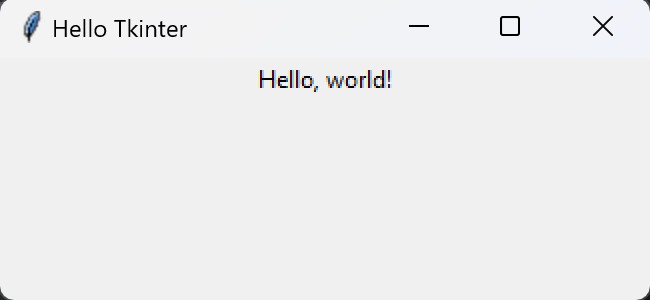
\includegraphics[width=\textwidth]{Images/TKinter/BasicWindows}
    \caption{\textbf{Basic Window}}
\end{figure}

\subsubsection{Button and Events}

Tkinter can create a window  and the button on the GUI. The following script shows a single button labeled "Click Me". When the button is clicked, "Button clicked!" is printed to the console.

\begin{itemize}
   
  \item button = tk.Button(root, text="Click Me", command=on\_click): Creates a Button widget, which is an interactive element that the user can click. The command=on\_click parameter links the button to the on\_click function, so when the button is clicked, the function is executed. This demonstrates event handling in Tkinter, similar to the action associated with the button in the second script. 
    
  \item button.pack(): Adds the button to the root window, arranging it according to the default layout provided by the pack() geometry manager. This places the button in the window, adjusting its size to fit the text "Click Me".
    
\end{itemize}

\begin{lstlisting}[language=Python]
    import tkinter as tk
    
    def on_click():
    print("Button clicked!")  # This function is called when the button is clicked.
    
    root = tk.Tk()
    button = tk.Button(root, text="Click Me", command=on_click)  # Creates a button. 'command' links the button to the on_click function.
    button.pack()
    
    root.mainloop()
    
\end{lstlisting}

\begin{figure}[h!]
    \centering
    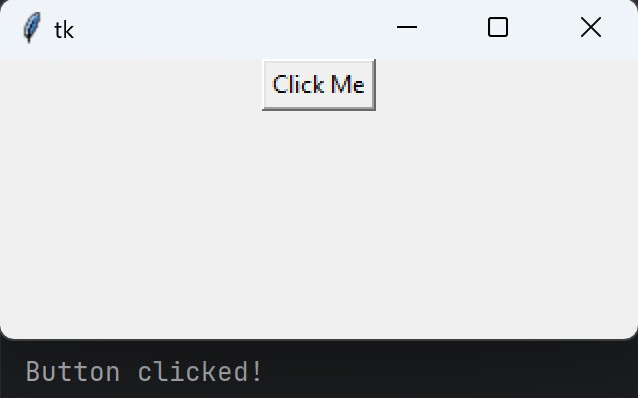
\includegraphics[width=\textwidth]{Images/TKinter/ClickMeButton}
    \caption{\textbf{Button}}
\end{figure}

\subsubsection{Entry Widget (Text Input)}

Tkinter can also create a text entry field and a submit button. When text is entered into the field and the submit button is clicked, the entered text is printed to the console.

\begin{lstlisting}[language=Python]
    
    import tkinter as tk
    
    def retrieve_input():
    input_value = entry.get()  # Retrieves text from the entry widget
    print(input_value)
    
    root = tk.Tk()
    entry = tk.Entry(root)  # Creates a text entry widget
    entry.pack()
    
    submit_button = tk.Button(root, text="Submit", command=retrieve_input)  # Button to trigger text retrieval
    submit_button.pack()
    
    root.mainloop()
    
\end{lstlisting}

\begin{figure}[h!]
    \centering
    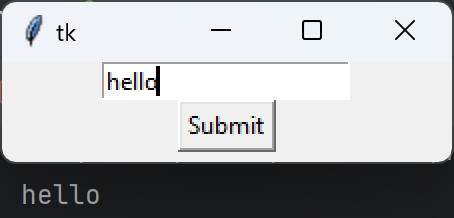
\includegraphics[width=\textwidth]{Images/TKinter/EntryValueOutput}
    \caption{\textbf{Entry Values and Result}}
\end{figure}

\subsubsection{Using Frames to Organize Layout}

The example below would like to show a window with two sets of buttons. The first set, on the top, contains a red and a green button side by side. The second set, at the bottom, contains a single blue button. This demonstrates the use of frames to organize widgets and the 'pack' geometry manager to arrange widgets within their parent container.

\begin{itemize}
    \item 1
\end{itemize}

\begin{lstlisting}[language=Python]
    
    import tkinter as tk
    
    root = tk.Tk()
    frame = tk.Frame(root)  # Creates a frame widget which will hold other widgets
    frame.pack()
    
    bottom_frame = tk.Frame(root)  # Another frame for separate grouping
    bottom_frame.pack(side=tk.BOTTOM)
    
    red_button = tk.Button(frame, text="Red", fg="red")  # 'fg' changes the button text color
    red_button.pack(side=tk.LEFT)
    
    green_button = tk.Button(frame, text="Green", fg="green")
    green_button.pack(side=tk.LEFT)
    
    blue_button = tk.Button(bottom_frame, text="Blue", fg="blue")
    blue_button.pack(side=tk.BOTTOM)
    
    root.mainloop()
    
\end{lstlisting}

\begin{figure}[h!]
    \centering
    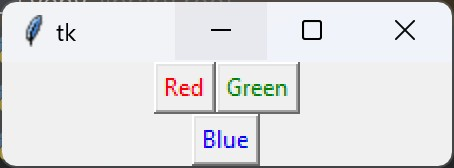
\includegraphics[width=\textwidth]{Images/TKinter/FrameLayout}
    \caption{\textbf{Frame Layout Example}}
\end{figure}

\subsection{Handling Files in Tkinter}

You can generally incorporate standard Python file handling methods and Tkinter GUI components. Here's a brief snippet to illustrate combining file operations with Tkinter:

\begin{enumerate}
    
    \item \subsubsection{Open Files}
    \texttt{filedialog.askopenfilename()} displays a file dialog to the user. This method returns the path to the selected file as a string. If the user cancels the operation (i.e., the return value is empty), the function returns early without doing anything.
    
    If a file is selected, the function opens the file in read mode ("r") and reads its content using input\_file.read(). It then prints the content to the console. In a full application, you might display this content in the GUI instead.
    
    \item \subsubsection{Create the basic window \ref{BasicWindow}}
    
    Similar as the previous section\ref{BasicWindow}, the main application window should be created to form the UI and also the buttons inside the window. \texttt{root = tk.Tk()} creates the main application window. \texttt{open\_button = tk.Button(...)} creates a button labeled "Open File". When clicked, it calls the open\_file function. \texttt{open\_button.pack()} adds the button to the main application window.
    
\end{enumerate}

\begin{lstlisting}[language=Python]
    
    import tkinter as tk
    from tkinter import filedialog
    
    def open_file():
    filepath = filedialog.askopenfilename()
    if not filepath:
    return
    with open(filepath, "r") as input_file:
    print(input_file.read())
    
    root = tk.Tk()
    open_button = tk.Button(root, text="Open File", command=open_file)
    open_button.pack()
    
    root.mainloop()
    
\end{lstlisting}

\begin{figure}[h!]
    \centering
    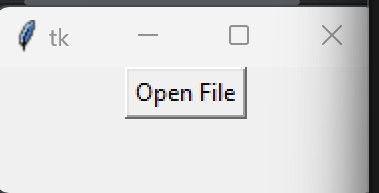
\includegraphics[width=\textwidth]{Images/TKinter/OpenFileFunction1}
    \caption{\textbf{Open File UI}}
\end{figure}

\begin{figure}[h!]
    \centering
    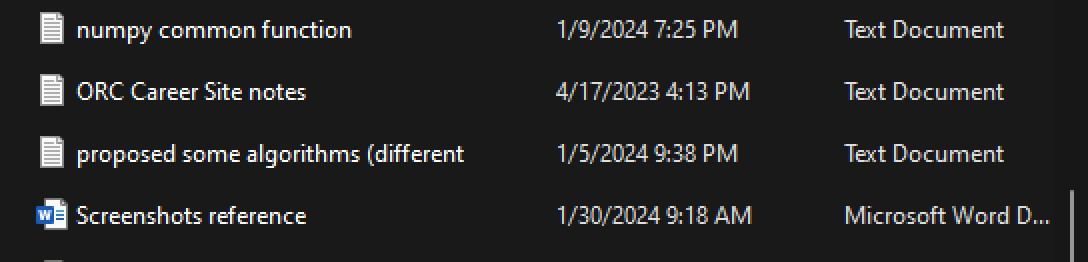
\includegraphics[width=\textwidth]{Images/TKinter/OpenFileFunction2}
    \caption{\textbf{File Selection}}
\end{figure}

\begin{figure}[h!]
    \centering
    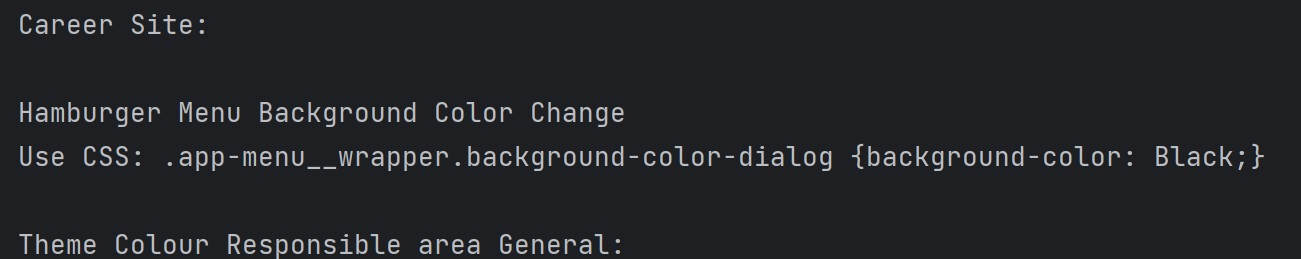
\includegraphics[width=\textwidth]{Images/TKinter/OpenFileFunction3}
    \caption{\textbf{Results shown in Console}}
\end{figure}

\subsection{Further Reading}

\subsubsection{Tkinter Documentation}

The official Python documentation provides a comprehensive guide to all aspects of Tkinter. Find it here : \url{https://docs.python.org/3/library/tkinter.html}

\subsection{pandas: a python data analysis library}

Offers tutorials and guides for Tkinter and Tk, covering both basic and advanced topics.
Find it here: \url{https://tkdocs.com/}

\subsubsection{Python and Tkinter Programming:Design and build functional and user-friendly GUI applications}

Due to its straightforward nature, Tkinter is a popular choice for creating Python GUIs. This book will guide you through the advantages and how to navigate the hurdles of Tkinter, enabling you to create sophisticated GUI applications.

In the second edition of "Python GUI Programming with Tkinter," you will not only gain an understanding of the Tkinter GUI framework but will also acquire essential skills for designing, developing, and maintaining extensive applications. Starting from the ground up, you will construct a comprehensive data entry application, adapting and enhancing your codebase to meet evolving requirements from users and the business.

Throughout the book, you will gain hands-on experience in managing the growing complexity of your codebase. You will explore beyond the basic functionalities of Tkinter widgets, employing strategies such as version control, unit testing, applying the MVC design pattern for clear separation of concerns, and leveraging object-oriented principles for streamlined code organization.
Find it here: \url{https://books.google.com.hk/books/about/Python_GUI_Programming_with_Tkinter.html?id=dS1LEAAAQBAJ&source=kp_book_description&redir_esc=y}


Remember to explore the official documentation first as it covers the most up-to-date information about Tkinter. The books, online resources,  mentioned above will complement your learning and provide additional insights into working with Tkinter.




